\documentclass[12pt]{report}

%Links
\usepackage[hidelinks]{hyperref}
\usepackage{xcolor}

%Lang
\usepackage[italian]{babel}
\usepackage[utf8]{inputenc}{\tiny }

%Math
\usepackage{amsfonts}
\newcommand{\graffe}[1]{\left\lbrace #1 \right\rbrace}

%Toc
\setcounter{tocdepth}{2}

%Bib
\usepackage[numbers]{natbib}

%Graphics
\usepackage{graphicx}

\begin{document}
\section{Clustering}
La classificazione non-supervisionata, più spesso chiamata \textit{clustering}, consiste nel separare un insieme di dati non etichettati in insiemi, i \textit{cluster}, internamente omogenei.
\subsection{Ontologia}
\subsubsection{Obiettivi}
Gli obiettivi del clustering possono essere: la ricerca di conferma di ipotesi effettuate a priori, oppure esplorare lo spazio delle feature, per effettuare dei ragionamenti a posteriori. Può essere impiegato per effettuare delle statistiche differenziate su più gruppi, oppure per elaborare i dati differentemente a seconda del cluster a cui appartengono.
\subsubsection{Dati}
I dati in input sono detti \textit{pattern} e sono solitamente valori in uno spazio multidimensionale $\mathbb{R}^d$. Le caratteristiche dei dati significative per il clustering sono dette \textit{feature}: i \textit{pattern} possono essere presentati come array di \textit{feature} oppure le \textit{feature} possono essere proprietà calcolate a partire dai \textit{pattern}.
\subsubsection{Metrica}
Spesso, la diversità tra due pattern viene espressa come distanza all'interno dello spazio delle \textit{feature}: dovrà essere, quindi, definita la metrica di distanza da utilizzare (distanza euclidea, \textit{Manhattan}, \textit{Mahalanobis}, distanze di \textit{Minkowski}, \dots ).

\subsubsection{Algoritmo}
Per effettuare clustering esistono molti tipi di algoritmi, che si dividono principalmente in due classi: algoritmi gerarchici e algoritmi partizionali.

Gli algoritmi partizionali impongono una suddivisione dello spazio delle \textit{feature} in più sottoinsiemi, che sono i cluster: se ogni \textit{pattern} può appartenere ad un solo cluster si parla di \textit{hard clustering}, altrimenti, se ogni pattern può appartenere a più cluster con un grado di \textit{membership} si parla di \textit{soft clustering} o \textit{fuzzy clustering}.

Gli algoritmi gerarchici organizzano il dataset in una struttura ad albero dividendo cluster troppo disomogenei (algoritmi divisivi) o unendo cluster simili tra loro (algoritmi agglomerativi). I risultati del clustering gerarchico vengono rappresentati con un albero binario (o un dendrogramma) in cui il nodo radice è il dataset e le foglie sono gli oggetti: i nodi intermedi indicano le divisioni del dataset in cluster; il risultato finale del clustering si ottiene troncando il dendrogramma ad una certa altezza: si otterrà una foresta in cui ogni albero corrisponde a un cluster.

I vantaggi del clustering gerarchico sono l'indipendenza dall'inizializzazione e il fatto che non sia necessario specificare a priori il numero di cluster. Però, sono poco robusti (molto sensibili a rumore e agli outlier), non riconsiderano le scelte già fatte (l'errata classificazione di un punto non viene mai corretta), hanno costo computazionale almeno quadratico ($O(N^2)$) e tendono a creare cluster sferici e fenomeni di inversione.

\subsubsection{Validazione}
Qualsiasi sia la strategia utilizzata, devono essere applicate delle procedure consolidate di validazione del clustering, per confermare la fondatezza del risultato ottenuto.

\subsection{Quad-Tree Decomposition}
\begin{figure} \centering
	\caption{Esempio di utilizzo di \textit{quad-tree decomposition} per la compressione di un'immagine raster binaria}
	\label{fig:qtdecomp}
	\ \newline 
	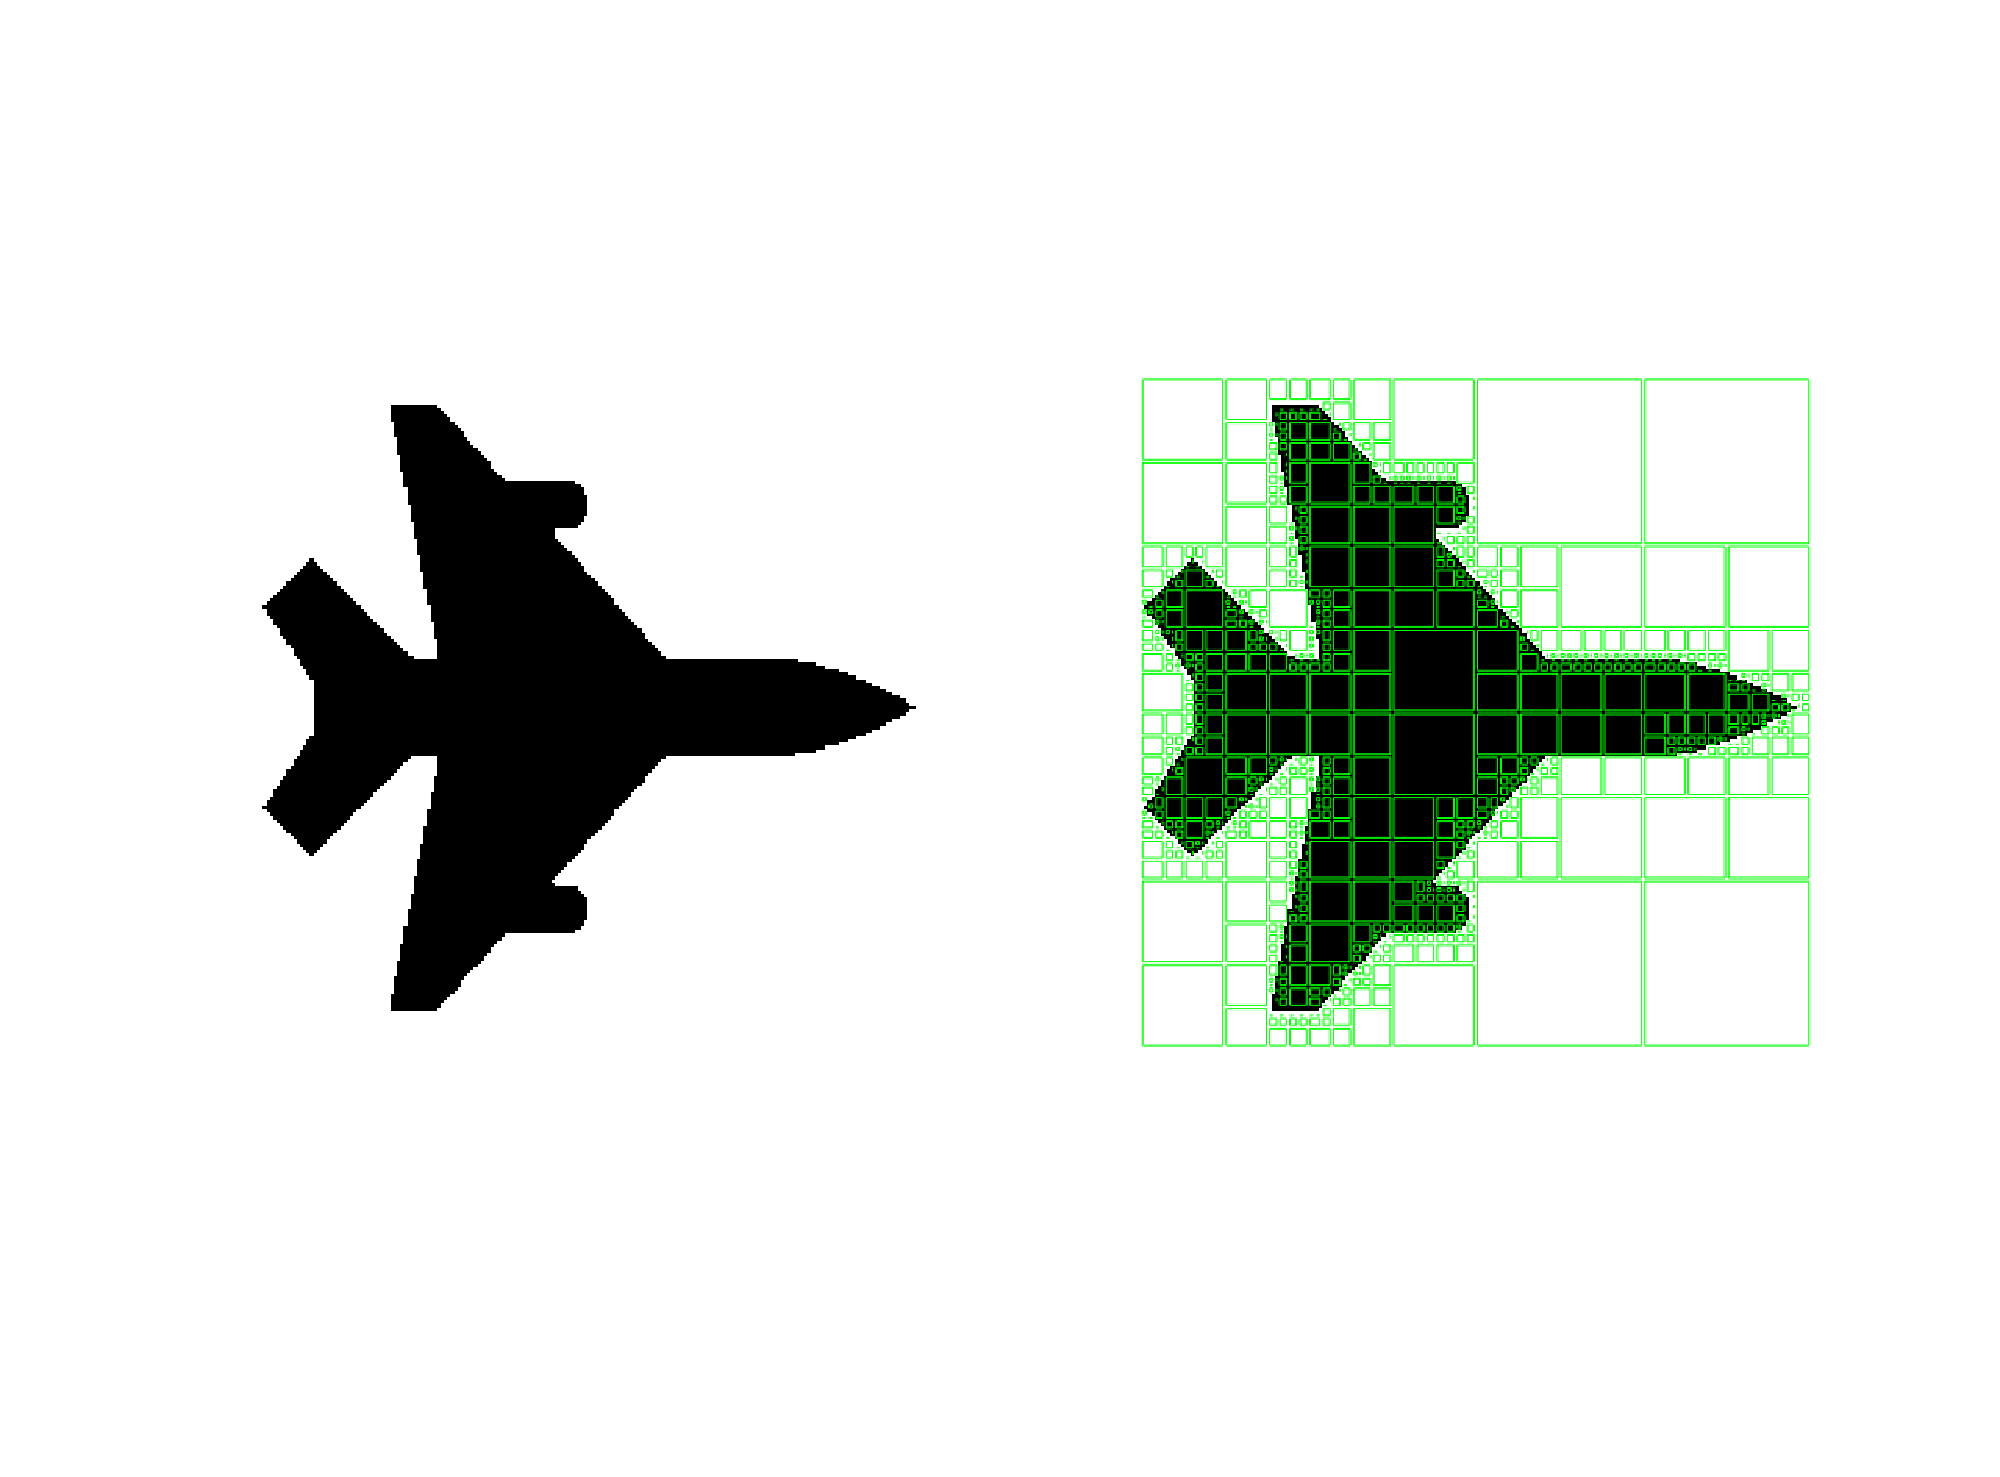
\includegraphics[width=\textwidth,trim={1.25in 2.5in 1.25in 2.5in},clip]{../images/qtdecomp.pdf}
\end{figure}
Con il termine \textit{quadtree} si indica una classe di strutture dati basate sulla decomposizione ricorsiva dello spazio: essi possono variare per il tipo di dati rappresentati, per il criterio che guida la decomposizione e la risoluzione (che può essere variabile o fissa). È un algoritmo gerarchico divisivo.

Il più comune approccio di tipo \textit{quad-tree decomposition} si basa sulla successiva divisione di un immagine in quattro quadranti di uguali dimensioni (come nell'esempio in figura~\ref{fig:qtdecomp}): un quadrante viene suddiviso solo se i pixel al suo interno sono disomogenei. Il nodo radice è l'intera immagine e il caso degenere della ricorsione è costituito dal singolo pixel (indivisibile). Occorre definire cosa si intende per disomogenei: per immagini binarie si può dire che ogni quadrante è omogeneo solo se tutti i pixel hanno lo stesso valore, per immagini RGB si può imporre una soglia di varianza.

\subsection{Agglomerative Clustering}
Il clustering agglomerativo si basa sulla seguente procedura \begin{enumerate}
	\item Ogni oggetto del dataset costituisce un singoletto (un cluster di un solo elemento). Si calcola la matrice di prossimità (la matrice che calcola per ogni coppia di cluster la distanza)
	\item Vengono combinati i cluster a distanza minima
	\item La matrice di prossimità viene aggiornata con le distanze tra il nuovo cluster e gli altri
	\item Se i cluster sono più di uno, ritornare al passo 2
\end{enumerate}
Gli algoritmi di clustering agglomerativo differiscono soprattutto per la politica di calcolo della distanza (oltre che per la funzione di distanza scelta) fra cluster, detta \textit{linkage}. Le più comuni sono\begin{itemize}
	\item \textit{Single linkage}: distanza minima tra oggetti dei due cluster
	\item \textit{Complete linkage}: distanza massima tra oggetti dei due cluster
	\item \textit{Group average linkage}: distanza media tra oggetti dei due cluster
	\item \textit{Median linkage}: distanza mediana tra oggetti dei due cluster
	\item \textit{Centroid linkage}: distanza tra i centroidi dei due cluster
	\item \textit{Metodo di Ward}: aumento di varianza \textit{whitin-groups}
\end{itemize}
Per ognuna di queste definizioni di \textit{linkage}, esistono dei pesi $\graffe{ \alpha_i , \alpha_j , \beta , \gamma }$, tali per cui il valore della distanza del nuovo cluster da uno degli altri cluster $C_l$ può essere ottenuto dai valori di distanza fra $C_l$ e i due cluster $C_i$ e $C_j$ che stiamo unendo, tramite la formula di ricorrenza di Lance e Williams:\\ \ \\
$ D(C_l,(C_i,C_j)) = $ 
\begin{flushright}
	$\alpha_i D(C_l,C_i)+ \alpha_j D(C_l,C_j) + \beta D(C_i,C_j) + \gamma \left| D(C_l,C_i)-D(C_l,C_j) \right| $
\end{flushright}
\begin{figure} \centering
	\caption{Esempio di dendrogramma risultante dal clustering agglomerativo degli stati membri degli USA per numero di arresti}
	\label{fig:hcdendrogram}
	\ \newline 
	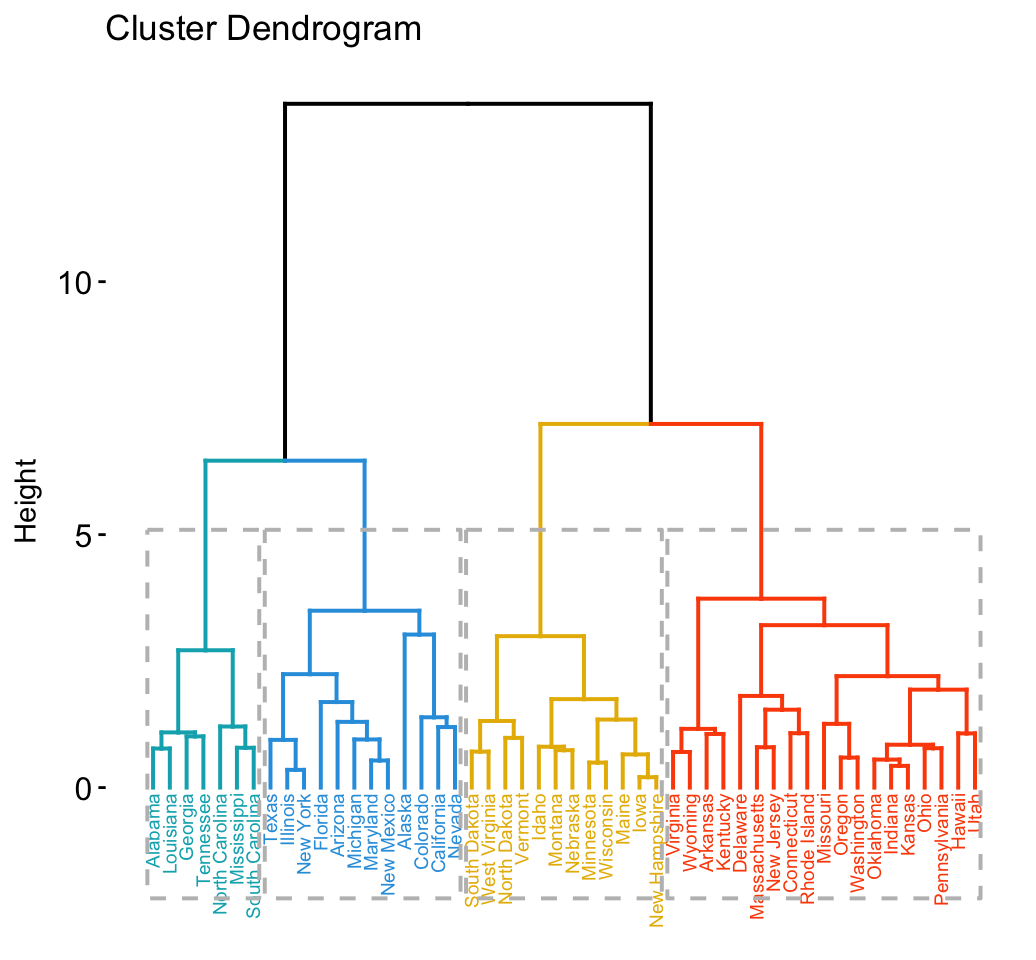
\includegraphics[width=0.75\textwidth,trim={1.5in 0.25in 0 1.25in},clip]{../images/hcdendrogram.png}
\end{figure}
I risultati del clustering agglomerativo vengono solitamente visualizzati con un dendrogramma (figura~\ref{fig:hcdendrogram}).

\subsection{K-means}
\begin{figure} \centering
	\caption{Esempio di applicazione di K-means: inizializzazione e risultato}
	\label{fig:kmeans}
	\ \newline 
	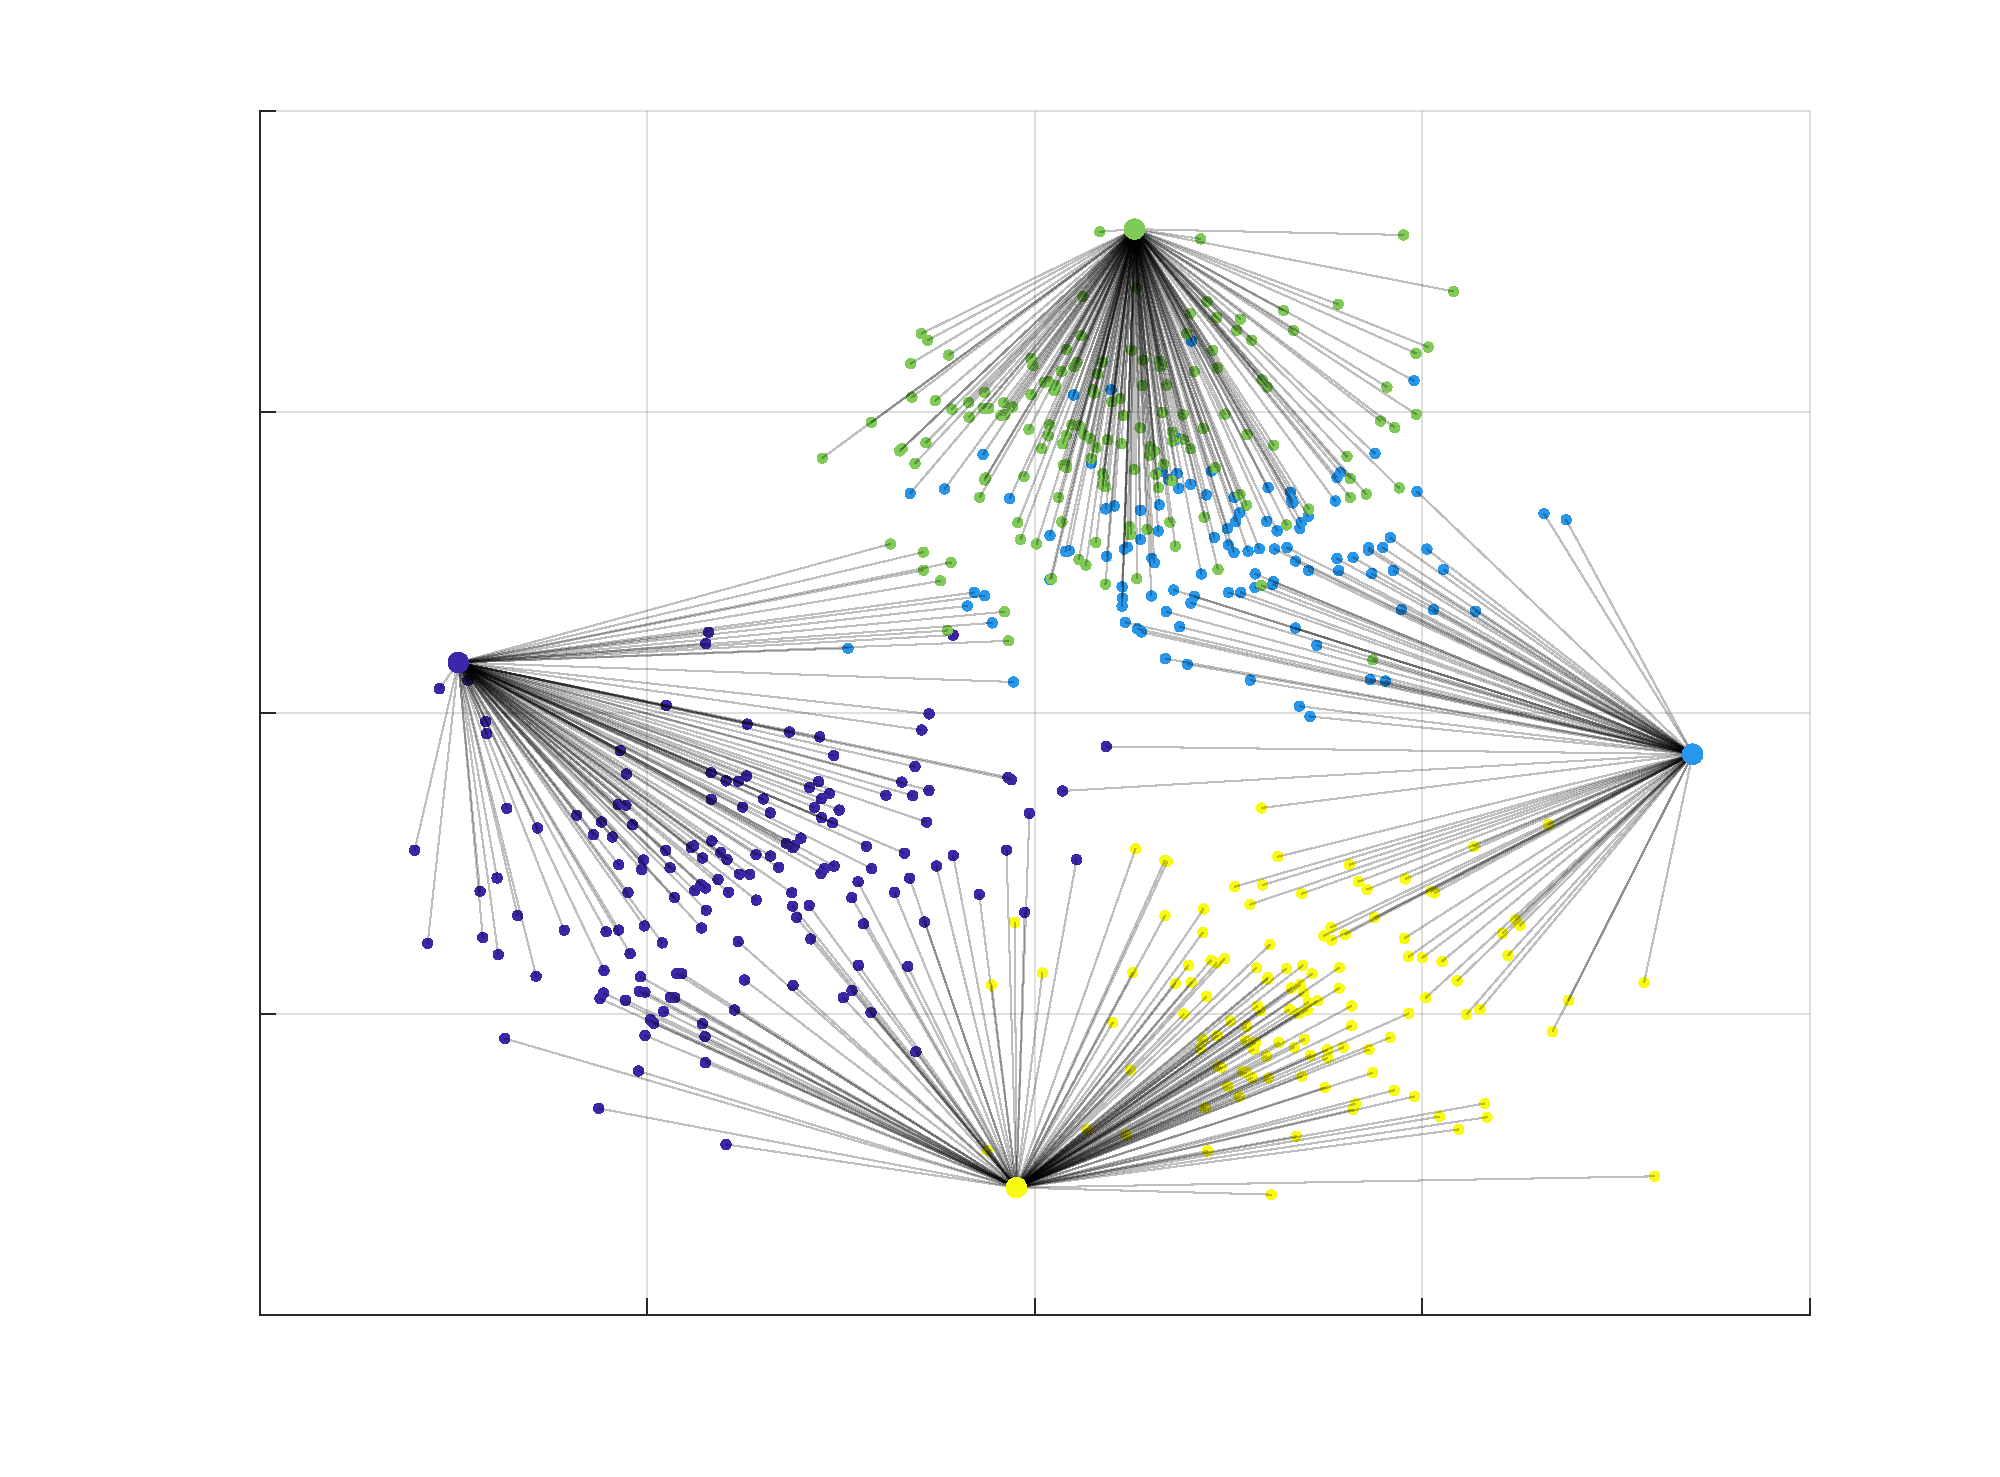
\includegraphics[width=0.49\textwidth,trim={2.5in 1.25in 1.5in 1.2in},clip]{../images/kmeans_0.pdf}
	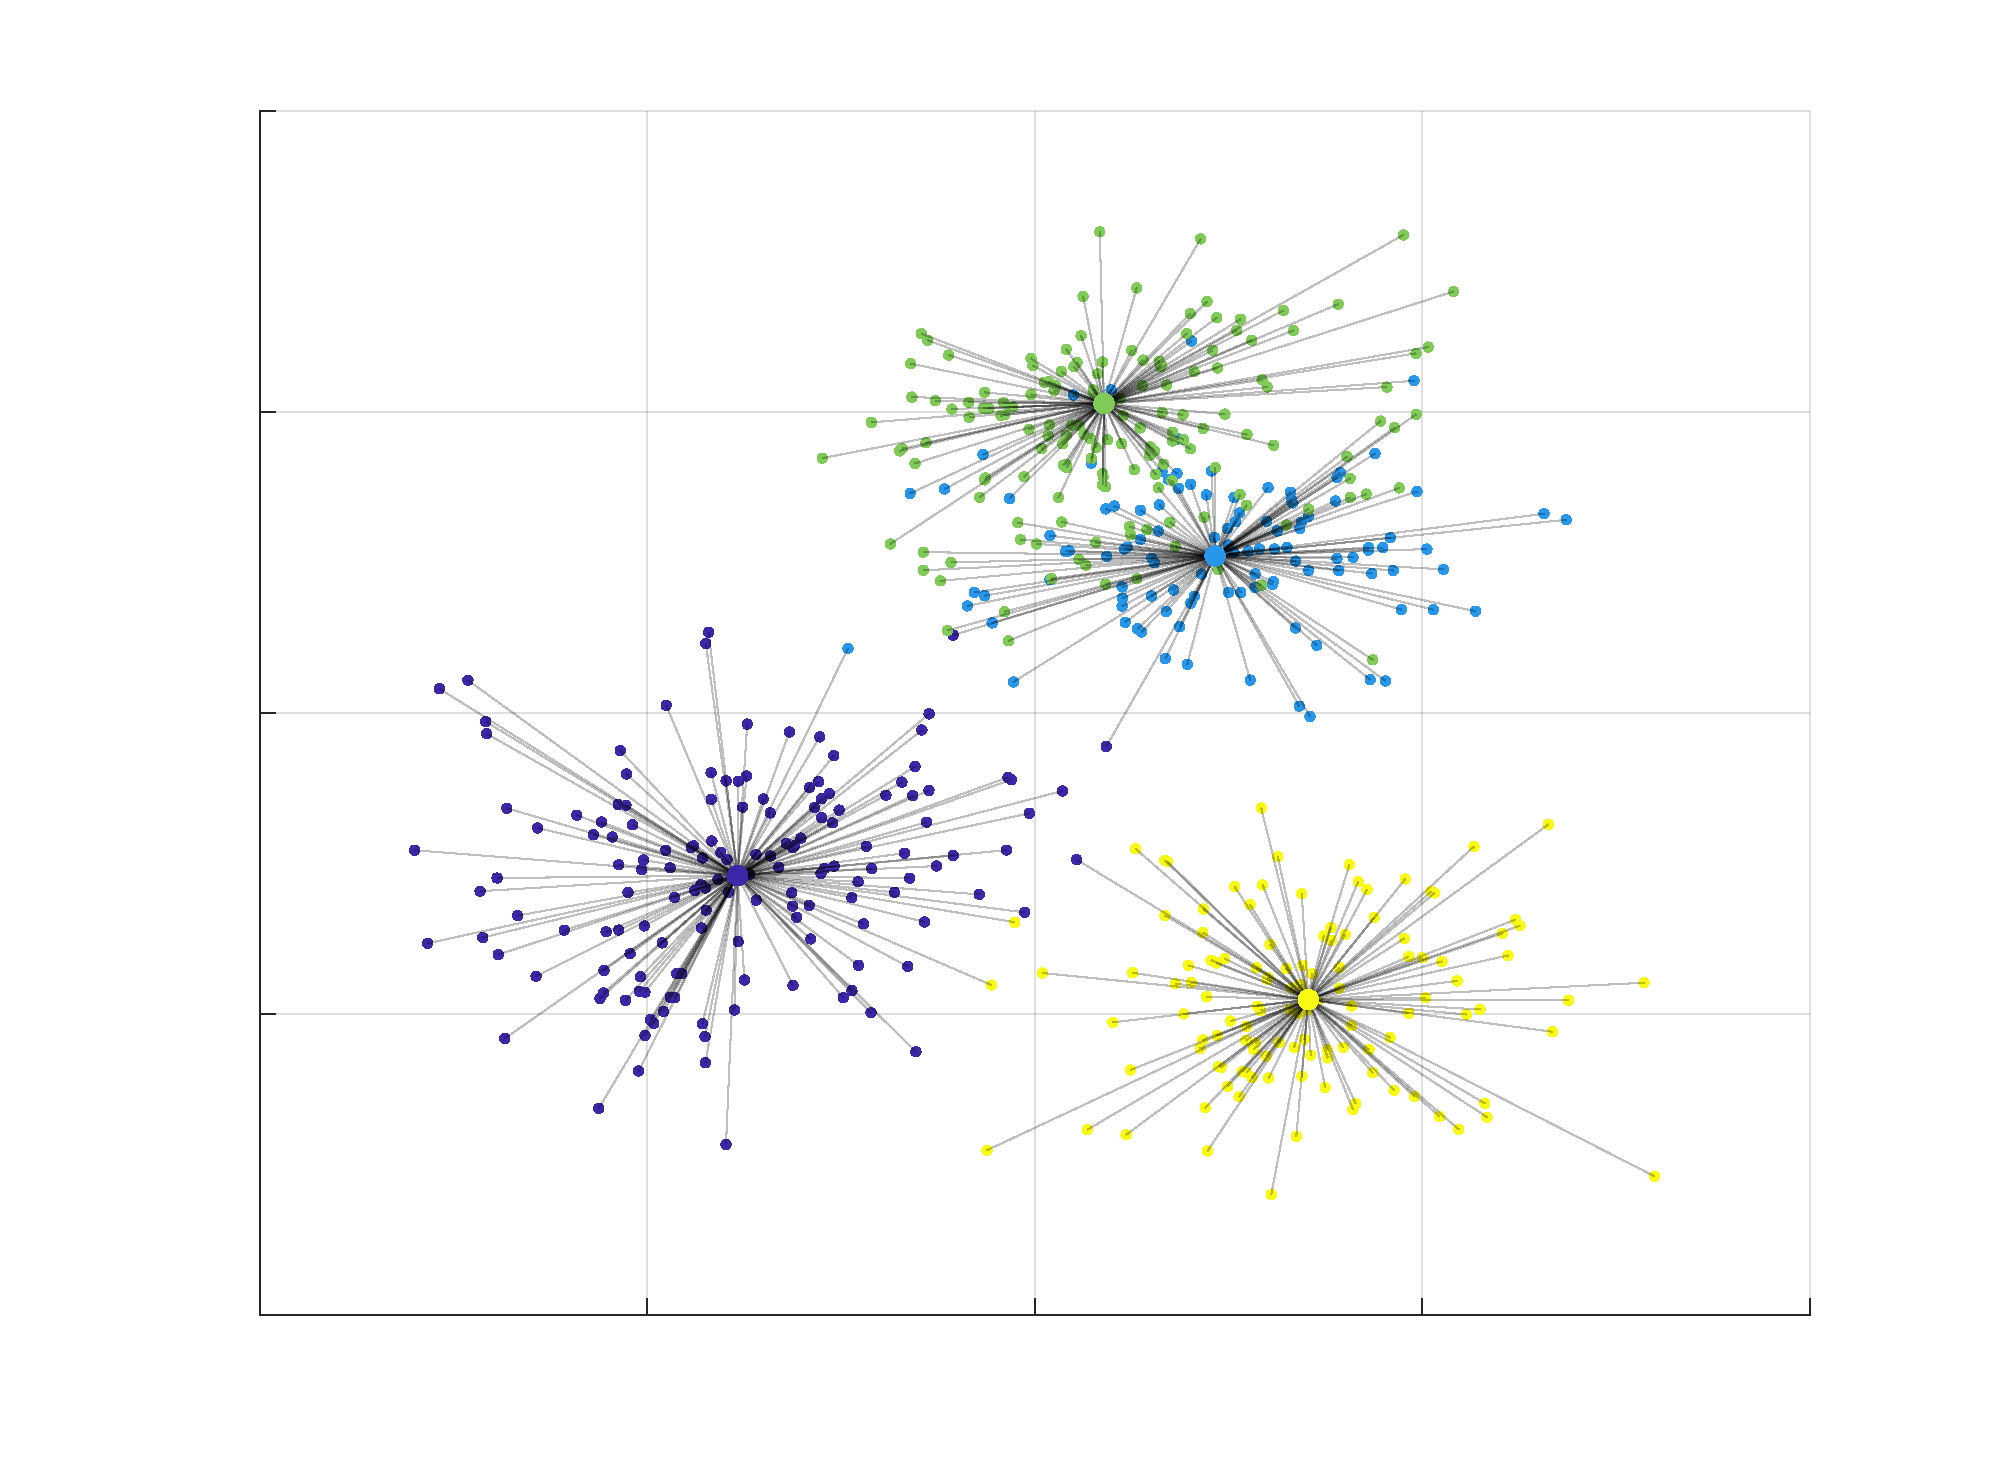
\includegraphics[width=0.49\textwidth,trim={2.5in 1.25in 1.5in 1.2in},clip]{../images/kmeans_f.pdf}
\end{figure}
Uno dei più famosi algoritmi di clustering è \textit{K-means}: è un algoritmo partitivo \textit{squared error-based}.\begin{enumerate}
	\item Viene inizializzata una partizione in K parti del dataset casualmente o in base a informazioni a priori, imponendo un prototipo per il clustering che è un vettore di medie
	\item Ogni oggetto viene assegnato al cluster più vicino
	\item Il vettore di medie viene aggiornato con le medie dei nuovi cluster
	\item Se il vettore è cambiato, tornare al punto 2
\end{enumerate}
Il cluster di appartenenza viene determinato come la media più vicina
$$ x_j \in C_w \Leftrightarrow ||x_j-m_w||<||x_j-m_i|| \ \forall i \neq w $$
K-means è molto semplice e si può implementare per risolvere problemi che coinvolgono grandi moli di dati (la sua complessità è lineare nel numero di pattern di input), inoltre, è estremamente parallelizzabile e lavora molto bene su cluster ipersferici.

Presenta vari svantaggi: non esiste un metodo universale ed efficiente per determinare le partizioni iniziali e il numero di cluster. Una strategia generale è di utilizzarlo più volte con inizializzazioni casuali, un'altra consigliata è il metodo di Kaufman. L'algoritmo iterativo non garantisce la convergenza in un ottimo globale: per ottenere ciò in modo efficiente, sono state sviluppate modifiche basate su tecniche stocasticamente ottime e algoritmi genetici.

Inoltre K-means è molto sensibile a rumore e agli outliers: algoritmi di tipo \textit{K-medoids} sono stati proposti, in cui i prototipi dei cluster sono scelti come i medoid dei cluster, ovvero i punti di ogni cluster che minimizzano la somma delle distanze dei punti del cluster dal medoid.

K-means ha anche il problema di basarsi sulla definizione di \textit{media}: non può essere applicato per tipi di dato sul quale non è possibile calcolare la media (o non avrebbe senso): in questi casi si può comunque usare K-medoids.

\end{document}